\capitulo{5}{Aspectos relevantes del desarrollo del proyecto}

En este punto se recoge de manera detallada y descriptiva el proceso seguido durante todo el proyecto. El orden de los puntos es cronológico, donde se habla acerca de las decisiones tomadas, los problemas surgidos y las posibles alternativas. 

Como aspecto importante, el objetivo inicial del proyecto era obtener la longitud del nervio, pero durante el transcurso del mismo, el odontólogo que da pie a este trabajo nos informó que lo importante era la longitud del diente, y no del nervio.

\section{Obtención de imágenes para entrenar}
Para empezar con el proyecto se contaba con tan solo 10 radiografías de la zona dental que se interesaba estudiar, además de los dos JSON correspondiente a cada radiografía que contenían los puntos del diente y del nervio segmentado.

El número de radiografías con las que se contaban era bajo, por lo que se decidió crear copias de las mismas, pero con diferentes modificaciones (proceso conocido como \emph{data augmentation}) para poder trabajar con un número de radiografías de las que se podría esperar buenos resultados. El tutor José Miguel había diseñado un \emph{notebook} encargado de realizar dicha función, de forma que, por cada radiografía original, se obtenían 11 (10 modificaciones y 1 original). Mi labor en dicho \emph{notebook} fue únicamente el de llevar a cabo una modificación para conseguir que las nuevas radiografías tuvieran el mismo tamaño que la radiografía original.

\subsection{Obtención de puntos de las imágenes modificadas}
Ahora que se contaban con las diferentes variaciones de las radiografías y de las diferentes máscaras del nervio y del diente, era turno de conseguir los puntos que delimitaban el borde de ambos elementos y almacenarlos en un JSON para poder trabajar con ellos.

Para ello se realizaron un total de 3 pruebas diferentes hasta que se obtuvo una forma de detectar los bordes de los dientes y nervios de forma precisa.

\subsubsection{Convex Hull}
La primera aproximación para obtener los puntos de las máscaras fue utilizar la técnica de \emph{convex hull}, o en español, envolvente convexa, pero que debido la propia expresión de la misma los resultados no fueron buenos, ya que las partes curvas no las detectaba del todo bien, como se aprecia en las Figuras \ref{f:diente} y \ref{f:nervio}.

\begin{figure}[h]
 \centering
  \subfloat[Diente]{
   \label{f:diente}
    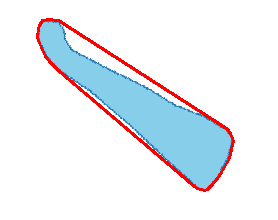
\includegraphics[width=0.5\textwidth]{img/CHDiente.png}}
  \subfloat[Nervio]{
   \label{f:nervio}
    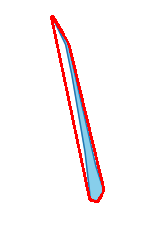
\includegraphics[width=0.3\textwidth]{img/CHNervio.png}}
 \caption{Ejemplo Resultados Convex Hull}
 \label{f:convex-hull}
\end{figure}

\subsubsection{OpenCV}
Tras los resultados, no muy buenos, obtenidos por el \emph{convex hull}, se estuvieron analizando diferentes alternativas. Una de ellas fue el uso de la biblioteca \emph{OpenCV} la cual tiene funciones implementadas para detectar bordes en imágenes y devolver todos los puntos que lo forman.

Los resultados que se obtuvieron fueron bastante buenos, aunque los bordes no eran de todo uniformes, como se puede apreciar en las Figuras \ref{f:diente2} y \ref{f:nervio2}.

\begin{figure}[h]
 \centering
  \subfloat[Diente]{
   \label{f:diente2}
    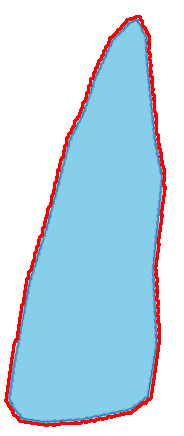
\includegraphics[width=0.2\textwidth]{img/CV2Diente.png}}
  \subfloat[Nervio]{
   \label{f:nervio2}
    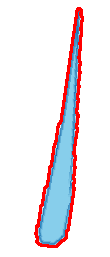
\includegraphics[width=0.12\textwidth]{img/CV2Nervio.png}}
 \caption{Ejemplo Resultados Bordes OpenCV}
 \label{f:cv2bordes}
\end{figure}

\subsubsection{Sckit-Image + OpenCV}
Pese a tener unos resultados bastante aceptables, se siguió investigando si existía alguna otra alternativa que mejorara los resultados anteriores. 

Tras analizar varias opciones, se decidió usar la librería \emph{Sckit-Image} para obtener una máscara de cada diente y nervio con la silueta del borde, donde los resultados eran bastante buenos.

\emph{Scikit-Image} no devuelve los puntos correspondientes al borde, sino una máscara binaria con dicha silueta. Es por ello, que para obtener los puntos correspondientes se volvió a utilizar la librería \emph{OpenCV}, donde ahora los bordes obtenidos sí que eran uniformes, como se puede ver en las Figuras \ref{f:diente4} y \ref{f:nervio4}

\begin{figure}[h]
 \centering
  \subfloat[Diente]{
   \label{f:diente4}
    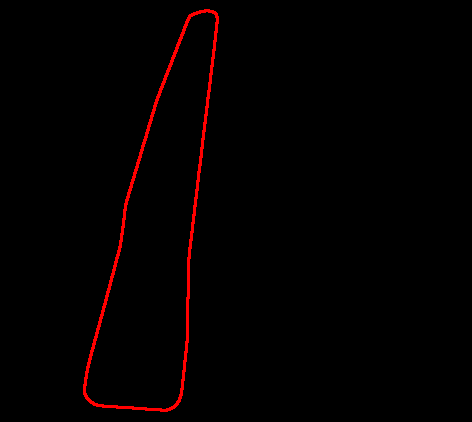
\includegraphics[width=0.5\textwidth]{img/SkiCv2Diente.png}}
  \subfloat[Nervio]{
   \label{f:nervio4}
    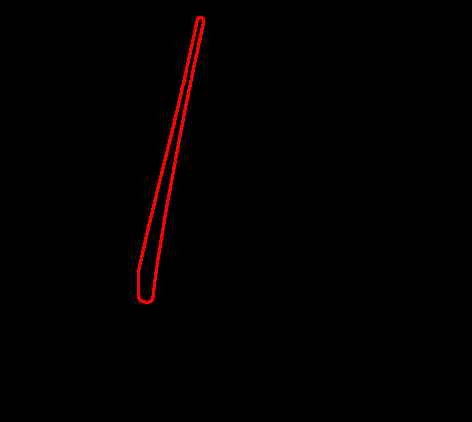
\includegraphics[width=0.5\textwidth]{img/SkiCv2Nervio.png}}
 \caption{Ejemplo Resultados Bordes Sckit-Image + OpenCV}
 \label{f:sskimage+cv2}
\end{figure}

\subsubsection{Problemas con los elementos en los bordes}
Para concluir con este punto, hay que hablar de un problema que había en algunas imágenes, donde el diente o el nervio estaba pegado al borde y la detección de los mismos no era correcta. La solución que se implementó fue la de añadir un borde blanco de 3 píxeles de ancho a todas las imágenes para evitar que los elementos estuvieran tocando el borde y la detección de los mismos fuera la correcta.

\section{Instalación Detectron2}
Ahora, que ya se contaba con un gran número de radiografías, gracias al \emph{data augmentation}, junto con sus JSON correspondientes a los puntos del nervio y del diente, era turno de instalar \emph{Detectron2} \cite{wu2019detectron2}.

Dicha tarea fue muy costosa, ya que no hay ninguna versión oficial para \emph{Windows}, aunque haya gente que sí lo ha conseguido instalar. 

Viendo que había gente que había tenido éxito, decidí crear un entorno en \emph{Anaconda} e intentar instalarlo. Dicha tarea fue imposible, puesto que constantemente salían errores nuevos hasta que llegué a un punto en el que no podía hacer nada para solucionarlo.

Tras los intentos fallidos, se utilizó temporalmente \emph{Google Colab} donde era sencillo de instalar y por el momento nos permitía seguir adelante. Pese a poder instalarse, los tiempos de ejecución eran demasiado elevados, por lo que se buscó como solución usar la máquina de la Universidad de Burgos, Gamma.

Finalmente, tras tener acceso a Gamma se consiguió instalar \emph{Detectron2} y se pudo empezar a trabajar en dicha máquina con unos tiempos de ejecución bastante bajos y muchos mejores que en \emph{Google Colab}.

\section{Construcción del modelo}
Ahora que ya se tenía instalado \emph{Detectron2} era momento de trabajar con el mismo. Debido a que \emph{Detectron2} es una biblioteca muy extensa y con muchas posibilidades. Se utilizó su \emph{notebook}, que tienen de ejemplo en \emph{Google Colab}\footnote{Ejemplo uso Detectron2: \url{https://colab.research.google.com/drive/16jcaJoc6bCFAQ96jDe2HwtXj7BMD_-m5}}, junto con una web\footnote{Web documentación Detectron2: \url{https://detectron2.readthedocs.io/en/latest/index.html}} que tenía todos las funciones  subdividas según sus funcionalidades, de forma que, según se necesitaba información de alguna cosa se recurría a dicha web, ya que tenía la documentación al completo.

Para obtener el modelo final se barajaron dos opciones:
\begin{itemize}
    \item Un modelo para detectar a la vez diente y nervio: consistía en un único modelo que, para cada radiografía, detectara a la vez el diente y el nervio de la misma (será la opción utilizada para llevar a cabo la aplicación).
    \item Un modelo para detectar el diente, y posteriormente otro modelo para detectar el nervio: se basaba en tener un modelo para detectar el diente de la radiografía, recortar dicha parte que contenía el diente, y finalmente tener otro modelo para detectar el nervio (esta opción se utilizó únicamente en las pruebas, ya que para calcular la longitud del diente era más sencillo poder acceder a las dos predicciones a la vez).
\end{itemize}

Los pasos seguidos para obtener el modelo en ambas opciones han sido:

\subsection{Distribución de las radiografías}
El primer paso fue dividir las diferentes radiografías en tres bloques diferentes: entrenamiento, validación y test. Para distribuirlas se hizo de forma aleatoria para no influir de ninguna manera, tanto positiva como negativamente, al modelo.

Los porcentajes de cada bloque fueron: 60\% entrenamiento, 20\% test y otro 20\% validación.

\subsection{Conversión JSON a COCO}
Para poder trabajar con imágenes segmentadas, \emph{Detectron2} necesita tener los datos en forma COCO, como ya se ha visto en la sección anterior \ref{COCO}.

Una vez ya se tenían los datos de forma correcta, se podían añadir cada dato a su correspondiente \emph{DataSet} (entrenamiento, test y validación).

\subsection{Entrenamiento}
Para realizar el entrenamiento, y con ello, obtener el modelo, se siguió la configuración recomendada en el \emph{notebook} de \emph{Detectron2} mencionado anteriormente. 

Además, se configuró el número de clases a predecir según las dos estrategias de modelo a conseguir. Para la opción de un único modelo tenía dos clases a predecir (diente y nervio), mientras que para la estrategia de dos modelos, cada uno de ellos tenía que predecir únicamente una clase (un modelo para el diente y otro modelo para el nervio).

\subsection{Predicción}
Una vez se obtuvo el modelo, era turno de realizar las predicciones. Para ello se usó el \emph{dataset} correspondiente a las imágenes de test. 

Adicionalmente, para analizar los resultados de las predicciones se utilizó IoU para conocer el porcentaje de similitud entre las predicciones y la segmentación real. Los valores mínimos, máximos y medios de los dientes y nervios obtenidos fueron los mostrados a continuación:

\begin{verbatim}
    DIENTES:
    La precisión media obtenida es de: 0.9284.
    La precisión mínima obtenida es de: 0.8487.
    La precisión máxima obtenida es de: 0.9793.
    
    NERVIOS:
    La precisión media obtenida es de: 0.8203.
    La precisión mínima obtenida es de: 0.5532.
    La precisión máxima obtenida es de: 0.9744.
\end{verbatim}

\section{Técnicas para medir la longitud del diente}
La forma de medir la longitud del diente a través de las predicciones obtenidas por parte de \emph{Detectron2} fue un proceso costoso ya que cuando se implementaba una técnica, se le mostraba al odontólogo y nos comentaba que no era muy adecuada.

Es por ello, que se han implementado un total de cuatro técnicas diferentes para medir el tamaño del diente.

\subsection{Técnica 1 - Longitud máxima del diente}
La primera aproximación fue obtener la distancia máxima entre la fila superior del diente y la inferior. Aparentemente, no da malos resultados como se puede apreciar en la Figura \ref{f:ejemplo1}, pero en aquellos dientes con cierta curvatura o inclinados la distancia no se calculaba de forma correcta.

\begin{figure}[h]
 \centering
  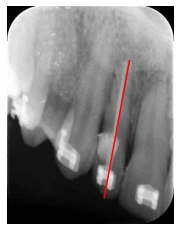
\includegraphics[width=0.35\textwidth]{img/Tecnica1.png}
 \caption{Ejemplo Resultado Técnica 1}
 \label{f:ejemplo1}
\end{figure}

\subsection{Técnica 2 - Skeleton del diente}
La siguiente técnica se basa en utilizar una función de la biblioteca \emph{Scikit-Image}, llamada \emph{skeleton} que devuelve una máscara binaria con los puntos centrales de un objeto. 

Por tanto, lo que hacía era calcular los puntos centrales del diente y posteriormente alargarlo hasta la fila superior e inferior del diente, Figura \ref{f:thin}.

Tras analizar los resultados obtenidos por dicha función, había casos en los que los puntos hacían una pequeña bifurcación al ensancharse el diente, por lo que se empleó una función muy similar, llamada \emph{thin} que eliminaba aquellos extremos que añadía \emph{skeleton}.

El problema de esa técnica es que alargar hasta la fila inicial y final del diente no era una buena idea, ya que había casos en los que los dientes, al tener una inclinación, el inicio y el fin del mismo, no se correspondía con dichas filas, como se puede apreciar en la Figura \ref{f:tecnica2}.

\begin{figure}[h]
 \centering
  \subfloat[Ejemplo Thin Diente]{
   \label{f:thin}
    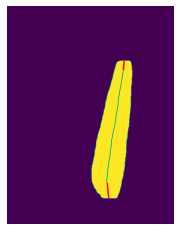
\includegraphics[width=0.35\textwidth]{img/Thin.png}}
  \subfloat[Resultado Final]{
   \label{f:tecnica2}
    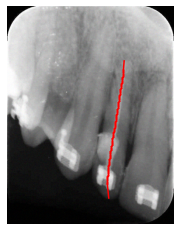
\includegraphics[width=0.35\textwidth]{img/Tecnica2.png}}
 \caption{Ejemplo Resultado Técnica 2}
 \label{f:ejemplo2}
\end{figure}

\subsection{Técnica 3 - Thinning del nervio}
La técnica 3 busca mejorar los problemas de la técnica anterior, de forma que en vez de aplicar el \emph{thinning} al diente se aplica al nervio, de forma que se consiguen unos puntos más precisos al encontrarse dicho nervio en la zona media del diente.

El operador morfológico \emph{thinning} funciona de igual forma que el \emph{skeleton}, solo que sobre los puntos obtenidos, por cada iteración, se borran los correspondientes a los bordes de forma que se finaliza el proceso una vez se pierde la conectividad.

Por otro lado, para alargar los puntos obtenidos hasta el diente, ahora se realiza cogiendo el primer y el último punto, se calcula la recta que pasa por ambos puntos y se alargar hasta el borde del diente, Figura \ref{f:alargada}. De esta manera se calcula la longitud del diente teniendo en cuenta su parte central independientemente de la inclinación del mismo.

La ecuación de la recta que pasa por dos puntos, $A(x_a,y_a)$ y $B(x_b,y_b)$ es:
$$\frac{x-x_a}{x_b-x_a}=\frac{y-y_a}{y_b-y_a}$$

Podemos hallar la pendiente de la recta anterior, $m$, evaluando:
$$m=\frac{y_b-y_a}{x_b-x_a}$$

\begin{figure}[h]
 \centering
  \subfloat[Thin Alargado hasta el Diente]{
   \label{f:alargada}
    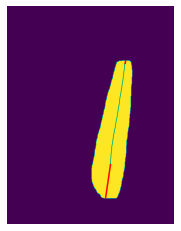
\includegraphics[width=0.35\textwidth]{img/Alargada.png}}
  \subfloat[Resultado Final]{
   \label{f:tecnica3}
    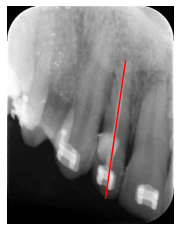
\includegraphics[width=0.35\textwidth]{img/Tecnica3.png}}
 \caption{Ejemplo Resultado Técnica 3}
 \label{f:ejemplo3}
\end{figure}

\subsection{Técnica 4 - Perpendiculares en el thin del nervio}
Tras mostrar los resultados obtenidos por parte de la técnica anterior al odontólogo, nos indicó que las mediciones eran correctas, menos en aquellos casos donde el nervio tenga una cierta curvatura, ya que no se tendría en cuenta.

Por tanto, esta técnica busca solucionar ese problema. Para ello, se realizarán perpendiculares a la recta obtenida por la técnica 3 en el \emph{thin} obtenido del nervio, de forma que se obtendrán los puntos de intersección, Figura \ref{f:inter}, y se irán sumando las distancias entre los puntos de corte.

Nuestro objetivo ahora es obtener rectas perpendiculares a las calculadas en el apartado anterior. Como sabemos el punto por el que han de pasar estas perpendiculares, basta calcular la pendiente, donde basta calcular:
$$m_{\perp}=\frac{-1}{m}$$

Donde $m$ es la pendiente de la recta obtenida en la técnica 3. 

Finalmente, a la suma total de los puntos de intersección se le sumará la longitud del final del \emph{thin} del nervio al punto final del diente (obtenido en la técnica 3), y de la misma manera, se sumará la distancia del punto inicial del diente (también obtenido en la técnica anterior) al punto inicial del \emph{thin}.

\begin{figure}[h]
 \centering
  \subfloat[Puntos de Intersección]{
   \label{f:inter}
    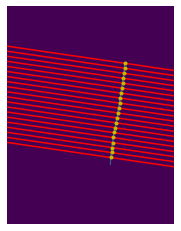
\includegraphics[width=0.35\textwidth]{img/Interseccion.png}}
  \subfloat[Resultado Final]{
   \label{f:tecnica4}
    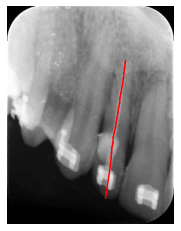
\includegraphics[width=0.35\textwidth]{img/Tecnica4.png}}
 \caption{Ejemplo Resultado Técnica 4}
 \label{f:ejemplo4}
\end{figure}

\subsection{Validación de los resultados}
Para poder validar la calidad de los resultados obtenidos se le solicitó al odontólogo que nos pasara la longitud de cada uno de los dientes de las radiografías que nos había proporcionado, junto con las longitudes, en milímetros, del ancho y del largo de cada radiografía para poder convertir la longitud de píxeles a milímetros. 

Pero a partir de aquí surgieron varios problemas. El primero de ellos fue que el odontólogo nos pasó la longitud real del diente y no la de la radiografía, que es siempre superior a la real, por lo que siempre los resultados obtenidos eran mayores.

El segundo problema era que, pese a saber lo que debería de medir en milímetros cada diente, los tamaños de las radiografías eran diferentes. Es decir, las radiografías que nos pasó el odontólogo no seguían las proporciones que deberían de tener en realidad, y pese a preguntar el porqué ocurría esto, el odontólogo nunca encontró una respuesta.

Por esta razón, los resultados obtenidos son siempre con unos errores relativos muy altos e inviables en la endodoncia (ya que el odontólogo quería que el error máximo fuera de 0.5 milímetros, puesto que si fuera superior se podrían causar daños irreparables en el paciente).

De modo que, nos hemos centrado más en comprobar que las segmentaciones de los dientes y nervios son buenas, junto con la técnica para calcular la longitud del diente y no tanto en el valor obtenido, ya que son valores que se alejan de la realidad y siempre van a dar resultados incorrectos.

\section{Desarrollo de la aplicación final del proyecto}
El último paso era desarrollar la aplicación final, puesto que ya que se contaba con el modelo encargado de realizar las predicciones y con una buena técnica para calcular la longitud del diente.

Para desarrollar la aplicación, inicialmente se barajó el instalar alguna biblioteca que permitiera lanzar una GUI desde \emph{Jupyter Notebook}. Se instalaron \emph{PySimpleGUI} y \emph{EasyGUI}, ya que tras analizarlas eran interfaces sencillas y fáciles de implementar.

Pero al tener alojada la aplicación en Gamma, nos encontramos con un problema , y es que en un servidor no se pueden lanzar GUI al no tener un \emph{display} asignado, como se aprecia a continuación: 

\begin{verbatim}
    TclError: no display name and no $DISPLAY enviroment
    variable
\end{verbatim}

Viendo que no se podían usar ninguna GUI, se optarón por dos opciones distintas:
\begin{itemize}
    \item  \emph{Google Colab}: hacer que la aplicación final fuese un \emph{notebook} en dicha plataforma, donde se trabajaría con el modelo obtenido en Gamma.
    \item  \emph{Ngrok}: emplear dicha herramienta para dar acceso a la aplicación de forma remota desde Internet y sin necesidad de estar conectado a Eudoram.
\end{itemize}

Pese a barajar ambas opciones, se llevaron a cabo las dos, ya que serían dos formas distintas de poder transmitir la aplicación del proyecto.

\subsection{Google Colab}
Para poder dar acceso en un \emph{notebook} a otro usuario es muy simple, ya que permite obtener un enlace a través del cual cualquier persona puede acceder y hacer funcionar la aplicación. 

\subsection{Ngrok}
Para poder utilizar \emph{Ngrok} era necesario instalar dicha herramienta en Gamma y crearse una cuenta en su web oficial\footnote{Ngrok: \url{https://ngrok.com/}} para poder obtener el toquen, Figura \ref{token}, que permite dar de alta la aplicación, Figura \ref{web}.

\begin{figure}[h]
    \centering
    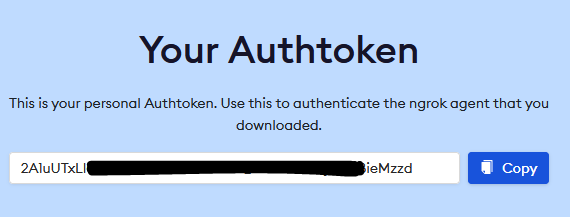
\includegraphics[scale=0.6]{./img/Token.png}
    \caption{Token de Usuario en Ngrok.}
    \label{token}
\end{figure}

\begin{figure}[h]
    \centering
    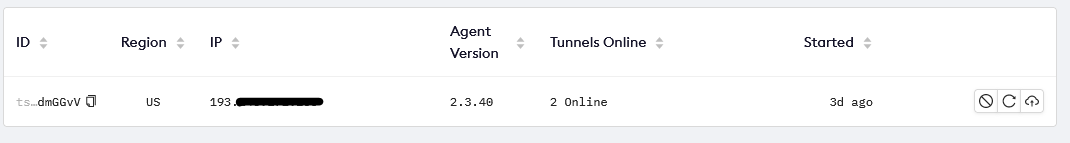
\includegraphics[scale=0.5]{./img/WebOnline.png}
    \caption{Ngrok con Web Activa.}
    \label{web}
\end{figure}

El uso del toquen es el de poder vincular una web pública a tu cuenta personal de \emph{Ngrok} para poder controlarla y gestionarla de una forma más cómoda. Además, también te permite tener acceso a las ventajas de tener una suscripción de pago, en caso de tener una activa.

Finalmente, tras implementar correctamente el modelo y sus diversas funcionalidades, los resultados que devuelve la aplicación se pueden apreciar en la Figura \ref{apli}.

\begin{figure}[h]
    \centering
    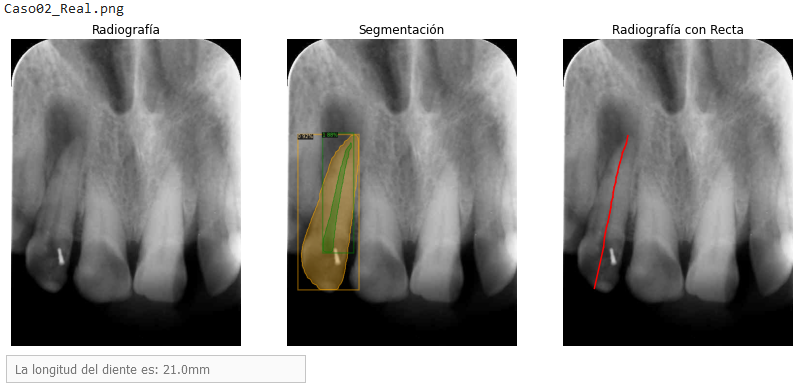
\includegraphics[scale=0.7]{./img/ResultadoApl.png}
    \caption{Resultado Aplicación Final.}
    \label{apli}
\end{figure}

\subsection{Acceso a la aplicación}
Los accesos a la aplicación del proyecto son:
\begin{itemize}
    \item \emph{Google Colab}:  \url{https://bit.ly/3R86dJc}
    \item \emph{Ngrok}:
    \begin{itemize}
        \item Web: \url{https://7b9a-193-146-172-150.ngrok.io}
        \item Contraseña acceso: \texttt{TfgUbu2122} 
    \end{itemize}
\end{itemize}
